\documentclass[10pt,a4paper]{article}
\usepackage{amsmath}
\usepackage[utf8]{vietnam}
\usepackage{amsfonts}
\usepackage{amssymb}
\usepackage{graphicx}
\usepackage[left=2cm,right=2cm,top=2cm,bottom=2cm]{geometry}
\setlength{\parindent}{0pt}
\begin{document}
\begin{center}
    \fontsize{30}{30}\selectfont
    KẾT QUẢ THỰC NGHIỆM
\end{center}
\fontsize{14}{20}\selectfont
Độ phức tạp thời gian: Theo thực nghiệm ta được độ phức tạp thời gian là $O(n^2)$
\begin{center}
     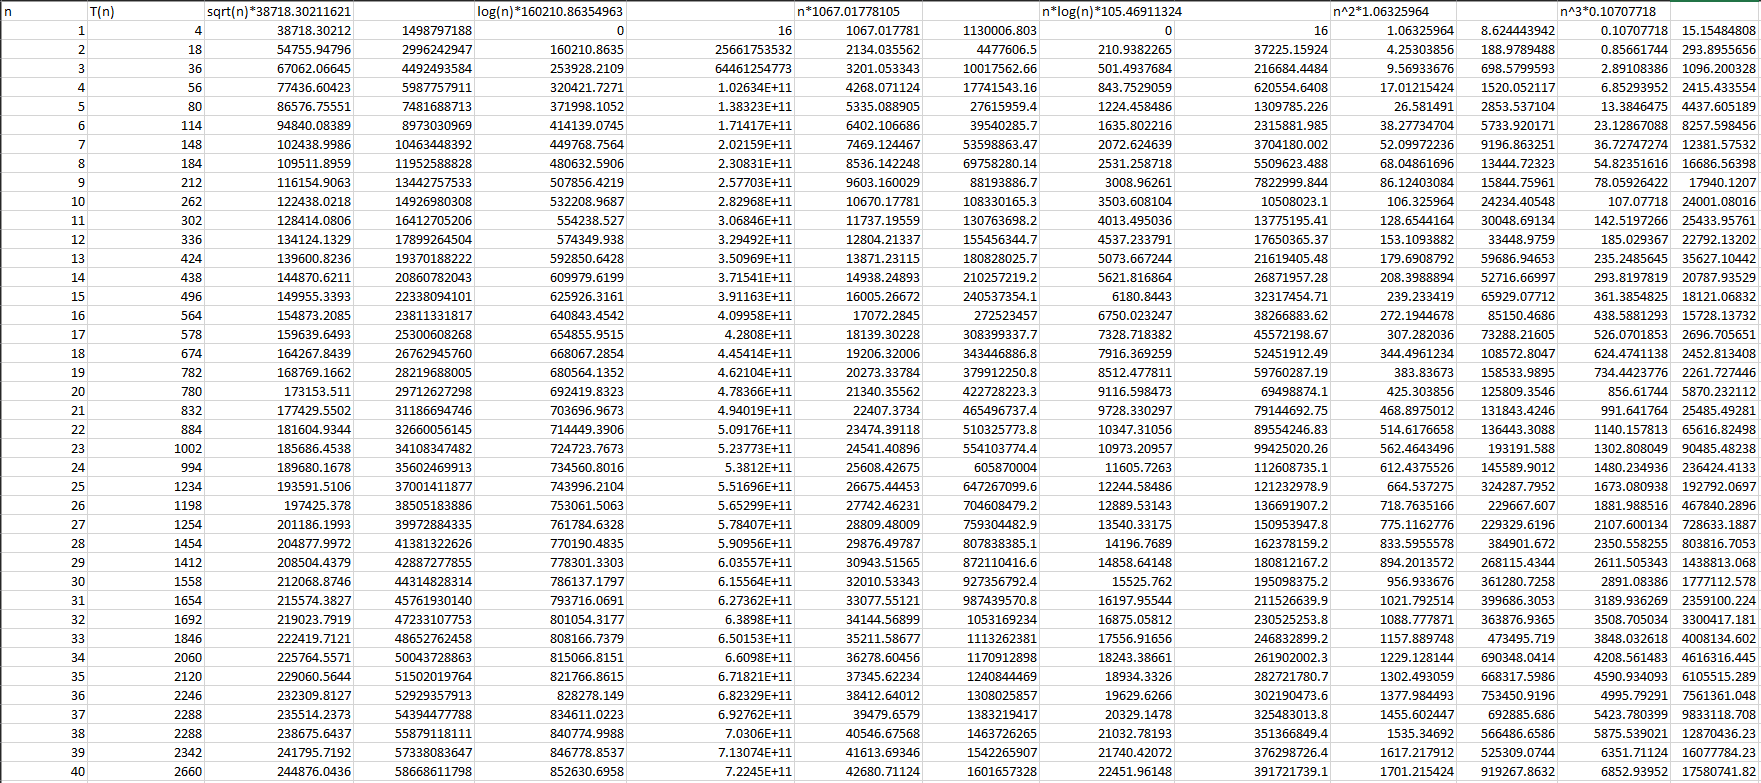
\includegraphics[scale=.45]{dpttg.png} \\
\end{center}
\vspace{1 cm}
Độ phức tạp không gian: Theo thực nghiệm ta được độ phức tạp không gian là $O(n^2)$
\begin{center}
     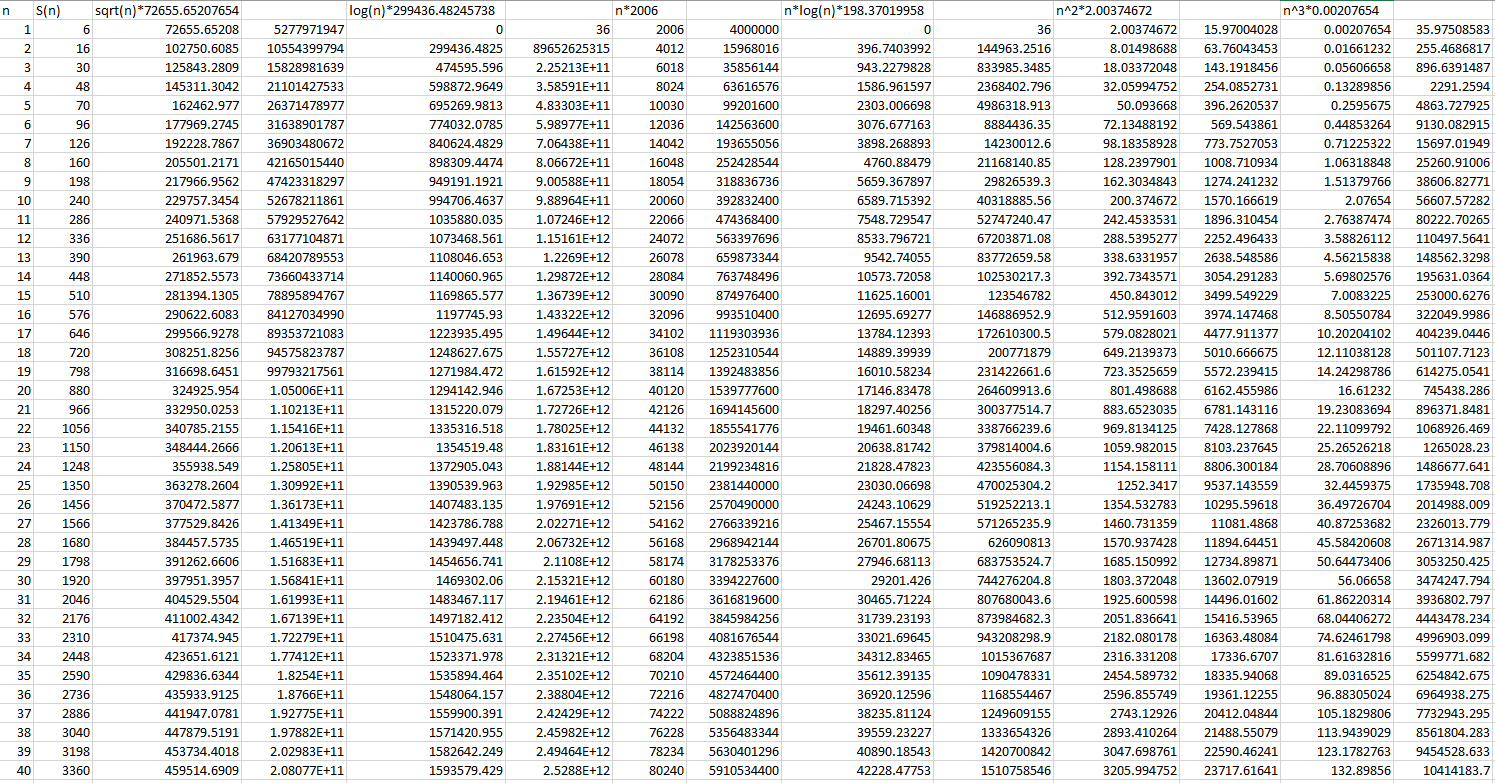
\includegraphics[scale=.5]{dptkg.png} \\
\end{center}
\end{document}
